\chapter{How to operate}
\chapter{Grammar school}

\begin{quote}
``... small number
of symbols and their grammar are enough to capture the huge
variety of equations...''
\end{quote}

The point of a variable is to replace it.  So in the formula 
$x(x+3)^2$ replacing $x$ for $7$ gives us $7(7+3)^2$.  
Yet even in the land of pure algebra where every symbol is variable it is absurd to
replace $+$ for $7$ to get $x(x73)^2$.   There is restraint in the substitution
of algebra built into what makes something an algebraic formula. When we pull 
on this thread we unravel an expansive relationship between free algebras and induction
and their role in computation.
% \medskip

% It is none other than grammar.

Consider how we know what to do when   
calculating $7(7+3)^2$.  For some of us a mnemonic springs to mind
(\emph{Please Excuse My Dear Aunt Sally}) or an acronym (PEMDAS).
These both unwind to tell us: Parenthesis Exponents Multiplication Division Addition Subtraction
in that order. This meandering thought process somehow elucidates how to read a formula. 
It gives the symbols complex structure that 
can be visualized with the following comic strip.
\begin{center}
    \begin{tikzpicture}[yscale=0.65]
        \node (A) at (0,0) {\begin{tikzpicture}[yscale=0.75]
        \node (f) at (0,0) {$7(7+3)^2$};
        \node[below of=f,scale=0.75] {$\times$};
        \node (x1) at (-1,-2) {$7$};
        \node (sqrt1) at (1,-2) {$(7+3)^{2}$}; 
        % \node[below of=sqrt1,scale=0.75] {$\circ$};
        \node (su) at (1.5,-3) {\textasciicircum $2$};
        \node (u) at (1,-4) {$7+3$};
        \node (x2) at (0,-6) {$7$};
        \node[below of=u,scale=0.75] {$+$};
        \node (three) at (2,-6) {$3$};
        % \node (x3) at (0,-8) {$x$};
        % \node (x4) at (2,-8) {$x$};
        % \node[below of=x2,scale=0.75] {$\times$};

        \draw[-] (f) -- (x1);
        \draw[-] (f) -- (sqrt1);
        % \draw[-] (sqrt1) -- (su);
        \draw[-] (sqrt1) -- (u);
        \draw[-] (u) -- (x2);
        \draw[-] (u) -- (three);
        % \draw[-] (x2) -- (x3);
        % \draw[-] (x2) -- (x4);

    \end{tikzpicture}};
    
    \node[right of=A,xshift=3cm] (B) {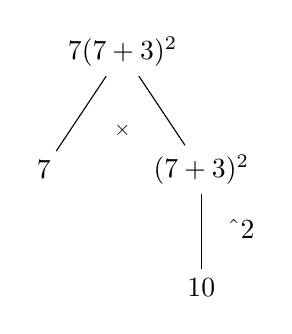
\begin{tikzpicture}[yscale=0.75]
        \node (f) at (0,0) {$7(7+3)^2$};
        \node[below of=f,scale=0.75] {$\times$};
        \node (x1) at (-1,-2) {$7$};
        \node (sqrt1) at (1,-2) {$(7+3)^{2}$}; 
        % \node[below of=sqrt1,scale=0.75] {$\circ$};
        \node (su) at (1.5,-3) {\textasciicircum $2$};
        \node (u) at (1,-4) {$10$};

        \draw[-] (f) -- (x1);
        \draw[-] (f) -- (sqrt1);
        % \draw[-] (sqrt1) -- (su);
        \draw[-] (sqrt1) -- (u);

    \end{tikzpicture}};
    
    \node[right of=B, xshift=3cm] (C) {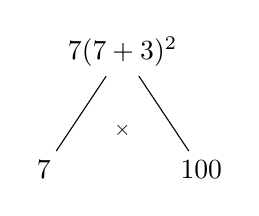
\begin{tikzpicture}[yscale=0.75]
        \node (f) at (0,0) {$7(7+3)^2$};
        \node[below of=f,scale=0.75] {$\times$};
        \node (x1) at (-1,-2) {$7$};
        \node (sqrt1) at (1,-2) {$100$}; 

        \draw[-] (f) -- (x1);
        \draw[-] (f) -- (sqrt1);

    \end{tikzpicture}};
    \node[right of=C,xshift=1cm] {$700$};

    \draw[thick] (A.north east) -- (A.south east);
    \draw[thick] (B.north east) -- (B.south east);
    \draw[thick] (C.north east) -- (C.south east);
\end{tikzpicture}
\end{center}
These step-by-step instructions start at the leaves $7$ and $3$ and join them as $7+3$ (computing $10$),
then the next step is to square (now $100$), then multiply by $7$, we reach $700$.
In hindsight, PEMDAS taught children a complicated form of induction.

\subsection{Induction \& Grammar}
You may have been taught induction through stories of falling 
dominos.  Good.  But what if induction was more like what we just did, climbing?
The domino illustration could bottle up the experience of climbing stairs.  
Now we climb trees and maybe mountains.
Setting up this induction was nothing more than a fragment of text but 
read through the lens of a grammar, e.g.\ PEMDAS, it came into a full form
as steps for recursion.

Parsing grammars in natural language is not always clarifying.  A simplistic
English grammar will often parse into cycles.
\begin{center}
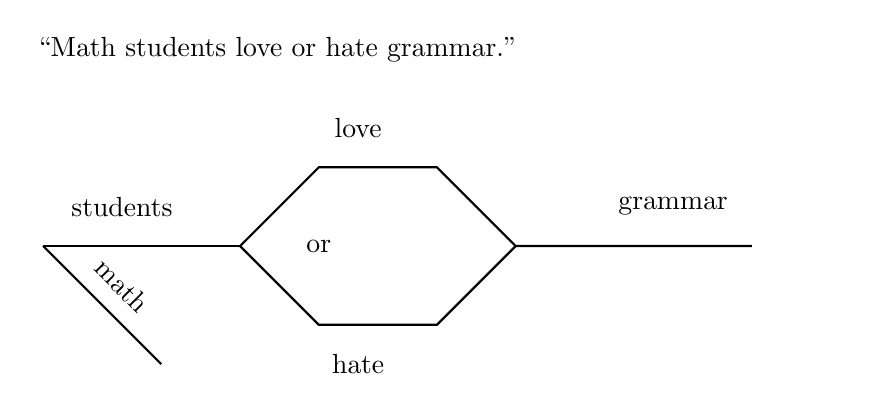
\begin{tikzpicture}
    \node[text width=4in] at (1,2) {``Math students love or hate grammar.''};
    \node at (-3,0) {students};
    \node[rotate=-45] at (-3,-1) {math};
    \node at (-0.5,-0.5) {or};
    \node at (0,1) {love};
    \node at (0,-2) {hate};
    \node at (4,0) {grammar};

    \draw[thick] (-4,-0.5) -- ++(2.5,0);
    \draw[thick] (-4,-0.5) -- ++(1.5,-1.5);
    \draw[thick] (-1.5,-0.5) -- ++(1,1) -- ++(1.5,0) -- ++(1,-1) -- ++(3,0);
    \draw[thick] (-1.5,-0.5) -- ++(1,-1) -- ++(1.5,0) -- ++(1,1);

\end{tikzpicture}
\end{center}
So our inductive climbs may one day need many routes, even go in cycles.
Fortunately, evaluating a formula has a precise algorithm without ambiguity. The
reason is that we had a rooted tree.  Trees have unique paths between any two
vertices. So if we start at the leaves we have a unique direction to reach the
root. 



\index{context-free}
That we got a tree in math formulas means we have a rather boring grammar, 
what Chompsky's \emph{Syntactic Structure} calls
\emph{context-free} grammars.\footnote{
    If an algebraist starts a talk with a story that ``...It was thought  all natural 
    languages were context-free until some obscure dialect in the alps or Africa was found...'', 
    then tune out until they return to equations.  
    Linguist never had such illusions. Even english is not context-free, read  James Higginbotham.} 
Don't be too disheartened.  Virtually every programming language has a 
context-free grammar and programs can communicate a lot of hefty ideas. 

\begin{quote}
    \textbf{Complex inductions can be specified by grammar.}
\end{quote}


\section{Valence}
\index{variadic}
We can add any finite list of $\sum_{i} n_i$ and 
programs back this up with commands like \code{sum(ns)} 
(the convention in programs is that a sequence $n_*$ is transcribed as 
the plural \code{ns}).  Likewise we can concatenate any 
number of strings.  In reality though, we have a limited work force:
ourselves and our machines. We therefore end up adding a bounded number at once,
often just 2.  So while we can entertain addition as having 
\emph{variadic} (variable valence), it is a practical reality that 
we build up arbitrary valance by composing several operators of 
fixed valence.

\index{bivalent!opeator}\index{binary operator|see{bivalent operator}}
Addition from here on out will be bivalent (also called binary), meaning 
that it requires 2 inputs.  We typically prefer infix grammar $\Box +\Box$.
Since we are evolving, we may as well permit multiplication as a bivalent operator
symbol, changing the signature to $\Box \cdot \Box$, i.e. $2\cdot 4$; or
$\Box\Box$, e.g. $xy$.   Avoid $\Box\times \Box$, we need that symbol elsewhere.
These days composition $\Box\circ\Box$ is written as multiplication; so, you can
use that symbol however you like.  Addition is held to high standards in algebra
(that it will evolve into linear algebra).  So when you are considering a binary
operation with few if any good properties, use a multiplication inspired
notation instead.   




\index{univalent!opeator}\index{unary operator|see{univalent operator}}
Valence 1, also called \emph{univalent} or \emph{unary}, operators include the negative sign $-\Box$ to create 
$-2$ as well as the transpose $A^{\dagger}$ of a matrix $A$.
Notice in the case of negative an integer remained an integer, but
 in the case of transpose a $(2\times 3)$-matrix becomes a $(3\times 2)$-matrix.   Operators can change the type of data we explore.
 
Programming languages add several others univalent operators
such as \code{++i, --i} which are said to \emph{increment} 
or \emph{decrement} the counter i (change it by $\pm 1$).

Programs also exploit a trivalent (ternary) operator:
\begin{center}
\begin{Pcode}[]
if (...) then (...) else (...)
\end{Pcode}
\end{center}
The words, while helpful, are unimportant and some languages
replace it with symbols emphasizing it is an operator:
\begin{center}
    \pcode{_?_:_}
\end{center}
Here for example is division with remainder of positive integers
\begin{center}
\begin{Pcode}[]
    div(m,n)=(m>=n)?(div(m-n,n)+(1,0)):(0,m)
\end{Pcode}
\end{center}

\section{Basic Grammar}
Admittedly  $\Box+\Box$, $\Box\cdot \Box$, and $-\Box$ indicate where to place 
information but they do not clarify what can be placed in each spot. 
We can add some clarity by clarifying the grammar with more meaningful tags.
For example, 
\begin{center}
    \code{<Matrix> ::= <Matrix> + <Matrix>}
\end{center}
would clarify that for this $+$ the intension was to add two matrices and 
the result will be another.   If we want to be certain that the dimensions 
match we can add this to the grammar.
\begin{quote}
    \code{<Matrix(2,3)> ::= <Matrix(2,3)> + <Matrix(2,3)>}\\
    \code{<Matrix(2,4)> ::= <Matrix(2,3)>  <Matrix(3,4)>}
\end{quote}
This approach becomes somewhat tedious as it depends so visibly on 
constants what will change between applications.  Later we revisit 
this problem with a few better options.


There are two implicit assumptions in what 
we have written.  First, while this definition is recursive we only intend 
that we should place a $+$ between two matrices that already exist.  In this 
way the grammar looks only back in time eventually settling on some constant
matrices.  Otherwise we could end up with some sort of infinite loop that 
never draws to a close.  Recursion that looks back in time to a start point is 
called \emph{primitive recursion}.  The second unexplained assumption is what 
qualifies as a constant matrix, a base case, to start the process off. 
The zero matrix for example would be one option, as would the matrices 
$E_{ij}$ that have $0$ in all position except row $i$ and column $j$ where 
the number is $1$.  If we include rescaling as an option then through 
linear combinations we could specify any matrix in this way.

Later we shall be more formal with grammars but we close we a few more 
demonstrations.
\begin{center}
\begin{Gcode}
<List> ::= cat <List> <List>
<List> ::= <List> + <List>
<A or B> ::= if <Boolean> then <A> else <B>
\end{Gcode}
\end{center}
When we wish to indicate that symbols $x$ have met the requirement to be 
treated as a type say ``matrix'', or ``list'', or ``Boolean'' we 
write $x:Matrix$, $x:List$, $x:Boolean$ accordingly.  We are also 
lenient with the use of popular shorthand such as $\mathbb{N}$ for natural 
numbers.  So $n:\mathbb{N}$ indicates that $n$ is a natural number.
Here are some related demonstrations.
\begin{quote}
    \code{(cat [1,2,3] [4,5,6]):List}.\\
    \code{([1,2,3] + [4,5,6]):\text{List}}.\\
    $\displaystyle 
        \begin{bmatrix} 1 & 0 & 8 \\ 2 & 7 & -1\end{bmatrix}
    + \begin{bmatrix} -1 & 0 \\ 0 & 1 \end{bmatrix}:\mathbb{R}^{2\times 3}$.
\end{quote}

\section{Operators to bring closure}
Sometimes we need operators to keep the data within some context.
For example we can multiply with rectangular matrices but their shape changes.
If we really plan a multiplication of $(2\times 3)$-matrices we need 
something unusual, like this:
\begin{align*}
    /A,B,C/ & = AB^{\dagger}C
\end{align*}
where $B^{\dagger}$ is the transpose.  This also has a partner.  If we have
$(3\times 2)$-matrices then the following product turns them into $(2\times 3)$-matrices.
\begin{align*}
    \backslash A,B,C\backslash & = A^{\dagger} B C^{\dagger}
\end{align*}
Playing these products off of one another leads to a fuller understanding of left-right 
behaviors of rectangular matrices.
Such products lead to the general 
concept of \emph{pair algebras}, e.g. pairing $\mathbb{R}^{2\times 3}$ 
with $\mathbb{R}^{3\times 2}$, which were introduced by Ottmar Loos in the 1970's.
\index{pair algebra}  
Pair algebras are the prefect place to study concepts like left/right pseudo-inverses $A^{\bot}$, resp. $A^{\top}$, of rectangular matrices $A$.
For example,
\begin{align*}
    \begin{bmatrix}
         1& 0 & 1\\
         -3 & 1 & 2
    \end{bmatrix}
    \begin{bmatrix}
        1 & 0\\
        3 & 1\\
        0 & 0 
    \end{bmatrix}
    & = 
    \begin{bmatrix} 1 & 0 \\ 0 & 1 \end{bmatrix}
\end{align*}
axiomatizes as the condition 
\begin{align*}
    /A,A^{\bot},A/&=A & \backslash A^{\bot},A,A^{\bot}\backslash =A^{\bot}.
\end{align*}
Pseudo-inverses are extensively used in Applied Mathematics to create 
solutions resilient to noise.

Another serious trivalent product comes up 
in symmetric matrices.  Notice if $A=A^{\dagger}$ and $B=B^{\dagger}$
then $(AB)^{\dagger}=B^{\dagger}A^{\dagger}=BA$ which is not in general 
the same thing as $AB$.  This means that the theory of symmetric matrices 
appears not to behave well under multiplication and that hampers attempts 
to study geometry and particle physics.

The solution comes in the form of other products, most importantly, 
the  \emph{Jordan Triple product} are the solutions to the equation
\begin{align*}
    2\{A,B,C\} & = ABC+CBA
\end{align*}
This is part of an whole family of Jordan products including solutions to
\begin{align*}
    2(A\bullet B) & = AB+BA\\
    2\langle A_1,\ldots,A_{\ell}\rangle & = A_1\cdots A_{\ell}+A_{\ell}\cdots A_1.
\end{align*}
Why the 2?  It is cosmetic but for example $I_n\bullet A=A=A\bullet I_n$ in this way. 
Notice in all these case if $A_i=A_i^{\dagger}$ then $\langle A_1,\ldots,A_{\ell}\rangle=
\langle A_1,\ldots,A_{\ell}\rangle^{\dagger}$. 
Pascual Jordan invented his products while formalizing 
Heisenberg's matrix model of quantum mechanics in the 1920's, and these were 
carefully investigated by Albert, von Neumann, Jacobson, culminating in the 
1994 Field's medal wining work of Efim Zelmanov.


A related product is to consider 
skew-symmetric matrices where $A_i^{\dagger}=-A_i$.  Then we would consider using the following 
alternating variation on the Jordan product known as a \emph{Lie bracket}
\begin{align*}
    [A,B]_+ & = AB-BA
\end{align*}
These operators are needed so that when we begin with a special type of
element---(skew) symmetric matrices, the product is again (skew) symmetric.
In the usual jargon we say that these matrices are \emph{closed} to the operator.
Sophus Lie studied the calculus of derivatives for its algebraic 
qualities in the 1880's.  These came to considerable fame with the rise of algebraic means to process 
geometry pushed along by Emile Cartan, Andre Weil, Dynkin, and the 2008 Abel prize winner Jacques Tits. 

When we can divide by 2, the Jordan and Lie perspectives become related.
\begin{align*}
    2AB = 2(A\bullet B)+[A,B].
\end{align*}
\section{Operators measuring defects}
Algebraist spend a lot of time worried about misbehaving operators 
causing them to generate new operators that spot the flaws.  This is another 
source of higher valence operators. If 
we can add, subtract, and multiply then we can make the following operators as well.
\begin{align*}
    [a,b] & = ab-ba \tag{Commutator}\\
    (a,b,c) & = a(bc)-(ab)c \tag{Associator}
\end{align*}
This commutator turns out to be the same as Lie's bracket and that coincidence 
has often been a subject to exploit.  Even so the goals are quite different. 
In Lie's case we need a product that respect skew-symmetry, we essentially forget 
the original matrix product and use just that Lie bracket.  Meanwhile when we 
approach this product as a commutator the entire purpose is to study the original 
product and gain insights by looking at the behavior of its commutator.

Commutative algebra requires $[a,b]=0$ while associative algebra needs $(a,b,c)=0$.
For example matrices fail to be commutative algebra but are associative.
Replace the role of multiplication of matrices with $[a,b]$ and ask for it's 
associate, i.e.
\begin{align*}
    (a,b,c)_{[,]} & = [a,[b,c]]-[[a,b],c]
\end{align*}
and we no longer get associative nor commutative algebra.  These are structures 
known as Lie algebras.  While not associative, because they are based originally 
on matrix products that are associative we can stumble eventually upon a 
graceful alternative
\begin{align*}
    0 & = [a,a] \tag{Alternating}\\
    0 & = [a,[b,c]]+[b,[c,a]]+[c,[a,b]].    
    \tag{Jacobi}
\end{align*}
So the problem is not getting worse, at least we wont be needing 
to look into some  valence 4 operators as defects.  Sabinin algebra 
studies how defects in operators pile up or die off.



Keep in mind requiring that $[a,b]=0$ or $(a,b,c)=0$ is an equation. 
Like any equation it has limited solutions.  By that reasoning, 
most of algebra wont behave commutative nor associative.

There are also variations on these.  If we have multiplication $\bullet$, 
an identity and inverses we can look for commuting products:
\begin{align*}
    [a,b]_{\bullet} & =(ab)^{-1}(ab)
    &
    {_{\bullet} [a,b]} & =(ab)(ab)^{-1}.
\end{align*}
These are especially useful in the  theory of equivalence, commonly subsumed 
in the topic of group theory and higher category theory.
Sometimes we have only left/right inverses so the same concept shifts to 
use these one-sided operators.
\begin{align*}
    [a,b]_{\bullet} & =(ab)\backslash (ab)
    &
    {_{\bullet} [a,b]} & =(ab)/(ab).
\end{align*}
These products emerge in the study of loops and combinatorics.


\section{Operators that unify}
Stranger ternary products showup in places where we wish we had easier binary products 
to explain things.  For example in geometry, part of the success of algebra and 
geometry was the realization that lines are described by the equations $y=mx+b$.
Yet that requires a number of hard to meet conditions on geometry beyond the obvious 
point-line intersection rules.  So when it comes to very general geometries 
it was not know how to describe lines algebraically as $y=mx+b$ because 
appropriate choices of $+$ and $\cdot$ were not known.
So Marshall Hall decided we could simply invent a trivalent (ternary) operator
\[
    -\otimes-\oplus -
\]
This is merely suggestive notation.  It allows us to write an equation 
that looks like our line equation:
\[
    y=m\otimes x\oplus b
\] 
yet this is not an amalgum of two operators just one single trivalent operator.
With this trivalent product, Hall was able to associate every 
projective plane to coordinates in some ``ternary ring''.  Once you have such a ternary ring you 
can go to work to see if it might actually decompose into two binary operations of multiplicaton 
and addition, e.g.\ by locating a ``one'' and a ``zero'' where $x=1\otimes x\oplus 0$.  Then 
you reverse the process and define $m\cdot x\defeq m\otimes x\oplus 0$ and $x+b\defeq 1\otimes x\oplus b$
to get a more familiar ring-like structure.





\section{Operators that guard}
When we divide we avoid division by $0$ (otherwise $0=0\frac{x}{0}=x$ so that every number
would be $0$ and we have no use for that sort of number system).  
Yet the problem is more pronounced.  With integers we cannot divide by anything other 
than $\pm 1$, so few that we in general through away division with integers.  
Now what happens in most of algebra is a mix of a good number of things with which we can 
divide but also a good number which we cannot use.  This means we cannot affort list 
the exception one by one, we need something stronger.

Consider matrices.  We decide if we can divide by $M$ if $\det(M)$ is invertible.
Here $\det$ is an operator on matrices.  It is an operator that informs us about 
what types of algebra we can perform on $M$.  It is \emph{guarding} us from mis using 
inverses.

A similar situation occurs with composing functions $f$ and $g$.  We need 
two guards: $\dom f$ and $\codom g$ that convert $f$ and $g$ to some other data 
where we can ask is $\dom f=\codom g$ and if so we get to use $f\circ g$.
The more algebraic operators we encounter the more often they are not total, 
meaning they cannot be applied everywhere, and the responsible step to take 
then is to add in further operators to serve as guards for when we can use the 
desired operations.

\section*{Conclusion}
A number of subtle problems are 
mounting.  For example, we probably want a Boolean (true/false) to 
go in the the left-most spot of an if-then-else-, and we cannot compose 
just any two functions and get expected results.  We scale a vector on one side 
by not the other.  Grammar must be more than just $\Box\cdot \Box$.

\section*{Exercises}

\begin{enumerate}
    \item Write down a grammar to accept natural numbers as digits.  Remember $07$ is not proper substitute for $7$.
    \item Make a grammar to describe rational numbers.
    \item Make a grammar to describe decimal numbers, call this \code{<Reals>}.  
    \item Augment your \code{<Reals>} to include constants for $\pi$ and $e$.
    \item Give a full grammar for real polynomials including conventional short-hand 
    such as $x$ for $x^1$ and $ax$ instead of $(a)(x)$.
    
    \item Suppose that we want to able to add a tally mark to either the left (L) or right (R).
    Define a grammar that allows.  Explain why this is not a model for the natural numbers.
        
    \item Turn the following function into code in both functional and procedural dialects.
    \begin{align*}
        f(n) & = \begin{cases}
                    0 & n=0\\
                    S0 & n=S(k)
        \end{cases}
         =\begin{cases} 0 & n=0 \\ 1 & \text{else}\end{cases}.
    \end{align*}
    
    \item Define multiplication of natural numbers from the Peano grammar given.
\end{enumerate}